% So we make this "beamer" rather than document!

\documentclass[11pt]{beamer}
% For handout add ,handout after 11pt

\usetheme[sectionpage=none,numbering=none]{metropolis}           % Use metropolis theme
	% To do printouts, add ", handout"  after aspectratio.
\usepackage{booktabs}
\usepackage{graphicx}
\usepackage{color}

\title{Black Boxes and Biased Implementations}
\author{\small Nick Eubank}
\date{\vspace*{.3in} \date}


% This is the beginning of a real document!
\begin{document}


\begin{frame}
\maketitle
\end{frame}

\begin{frame}[c]{Black Boxes}
What does it mean to be a Black Box algorithm?
\begin{itemize}
    \pause \item Not public (e.g. proprietary)
    \pause \item Not transparent (e.g. neural network)
    \pause \item Both
\end{itemize}
\end{frame}

\begin{frame}[c]{Black Boxes Hide...}
Proprietary:
\begin{itemize}
    \pause \item Can't evaluate accuracy issues
    \pause \item Can't evaluate coding / data errors
    \pause \item Can't tell if it's using factors we think are unjust \\
    Has mother been arrested?
\end{itemize}
\end{frame}


\begin{frame}[c]{Black Boxes Hide...}
Non-Transparent Models (SVMs, Neural Networks, etc.):

Even if public, these models have no constant marginal effects!
\vspace{0.1cm}
{\Large No $\frac{\partial Y}{\partial X}$!}\\
\vspace{0.1cm}
e.g.:
\begin{itemize}
    \item High School $\rightarrow$ College: \\
    Decreases probability of recidivism if 24
    \item High School $\rightarrow$ College: \\
    Increases probability of recidivism if 25
\end{itemize}
\end{frame}

\begin{frame}[c]{Black Boxes}
Factor Importance:
\begin{itemize}
    \item Contributions to predictive power, \emph{not}
    \pause \item Clear report of \alert{how} factor impacts outcomes
\end{itemize}
\pause Can get \emph{averages} of the data you have, which is fine for advertising...\\
But if errors send people to prison / prevent from getting medical treatment, not ok!
\end{frame}

\begin{frame}[c]{Interpretable Models}
\begin{figure}
  \centering
\pause 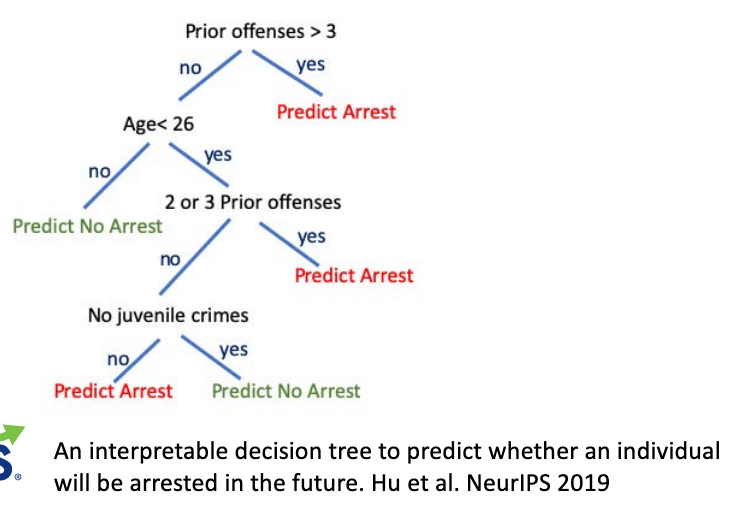
\includegraphics[width=\textwidth]{images/rudin_model_compas.png}
\end{figure}
\pause Don't preclude bias, but make models easier to audit!
\end{frame}

\begin{frame}[c]{Interpretable Models}
\begin{figure}
  \centering
\pause 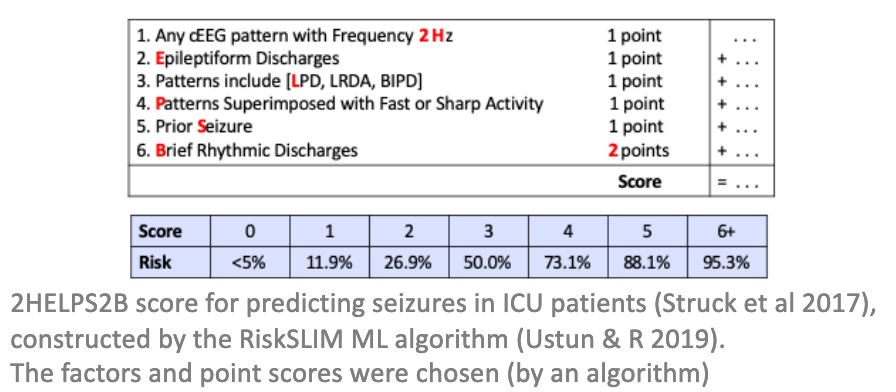
\includegraphics[width=\textwidth]{images/rudin_model_seizure.png}
\end{figure}
\pause Don't preclude bias, but make models easier to audit!
\end{frame}


\end{document}
